\documentclass[pdflatex,compress,mathserif]{beamer}

%\usetheme[dark,framenumber,totalframenumber]{ElektroITK}
\usetheme[darktitle,framenumber,totalframenumber]{ElektroITK}

\usepackage[utf8]{inputenc}
\usepackage[T1]{fontenc}
\usepackage{lmodern}
\usepackage[bahasai]{babel}
\usepackage{amsmath}
\usepackage{amsfonts}
\usepackage{amssymb}
\usepackage{graphicx}
\usepackage{multicol}
\usepackage{lipsum}

\newcommand*{\Scale}[2][4]{\scalebox{#1}{$#2$}}%

\title{PEMODELAN JARINGAN KOMUNIKASI}
\subtitle{The Life of a Packet}

\author{Tim Dosen Pengampu}

\begin{document}

\maketitle

\section{DNS - The Domain Name System}

\begin{frame}
	\frametitle{OSI Reference Model (Encapsulation)}
	\begin{center}
		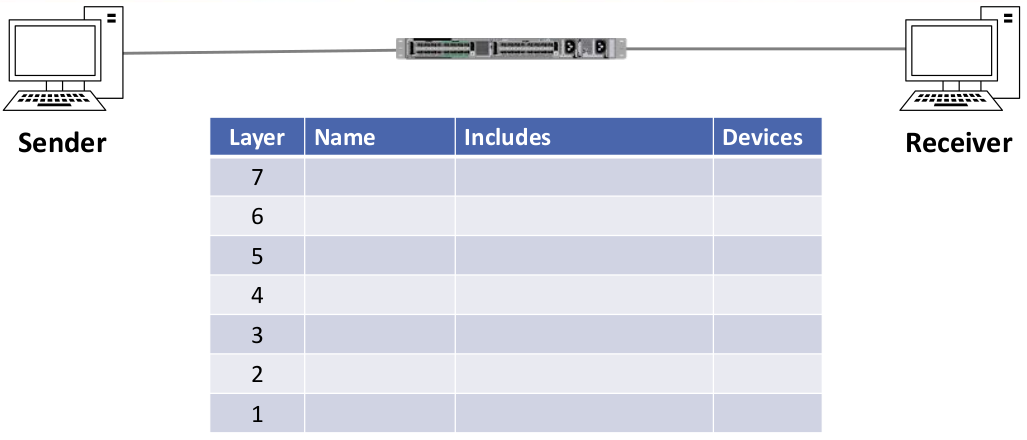
\includegraphics[width=\linewidth]{img/img01}
	\end{center}
\end{frame}

\begin{frame}{OSI Reference Model (Encapsulation)}
	\begin{center}
		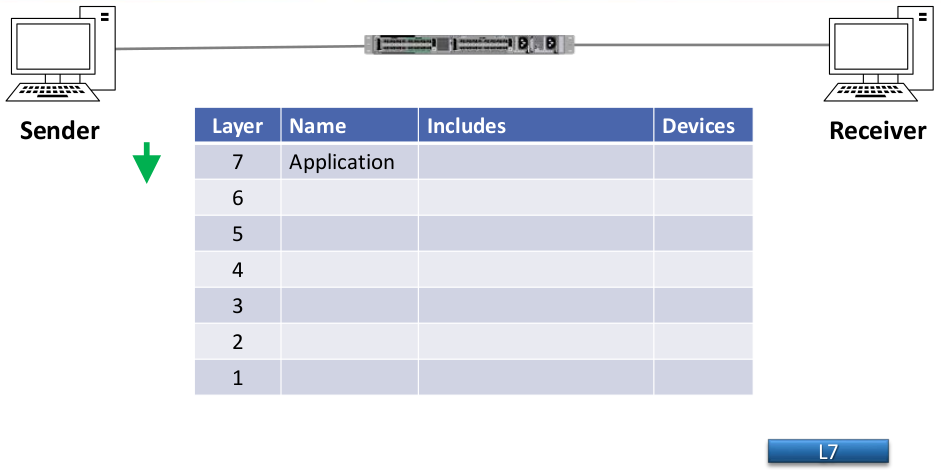
\includegraphics[width=\linewidth]{img/img02}
	\end{center}
\end{frame}

\begin{frame}{OSI Reference Model (Encapsulation)}
	\begin{center}
		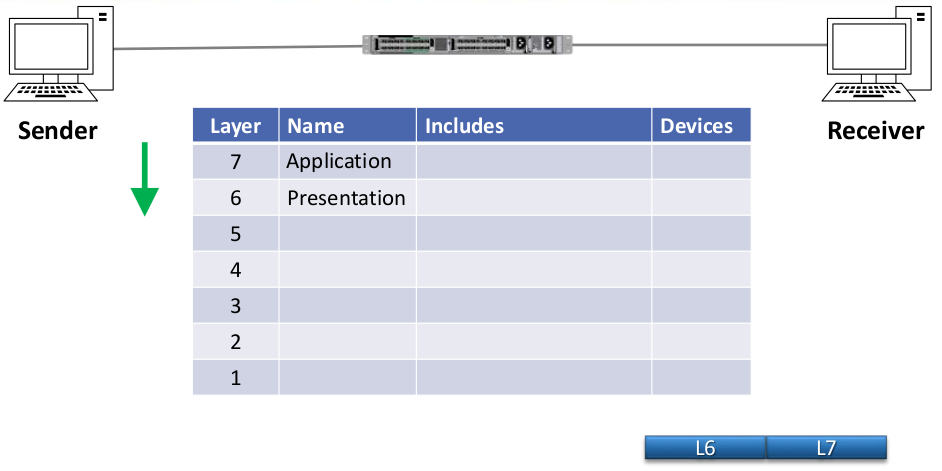
\includegraphics[width=\linewidth]{img/img03}
	\end{center}
\end{frame}

\begin{frame}{OSI Reference Model (Encapsulation)}
	\begin{center}
		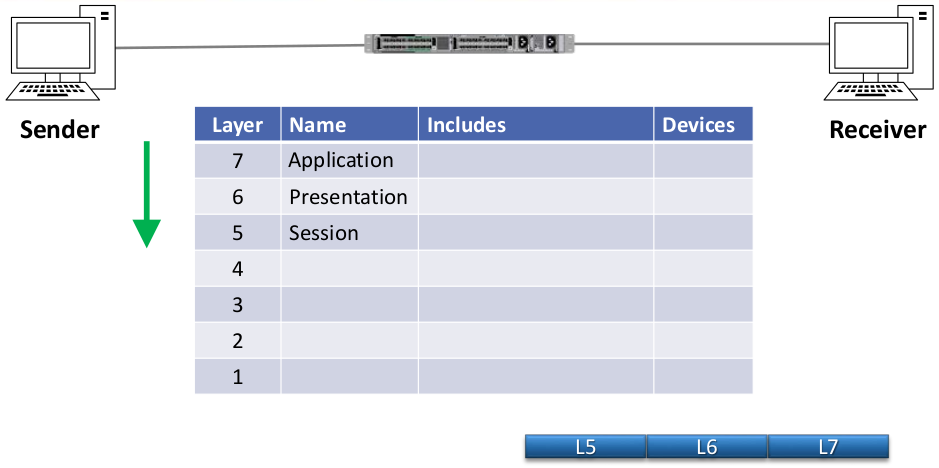
\includegraphics[width=\linewidth]{img/img04}
	\end{center}
\end{frame}

\begin{frame}{OSI Reference Model (Encapsulation)}
	\begin{center}
		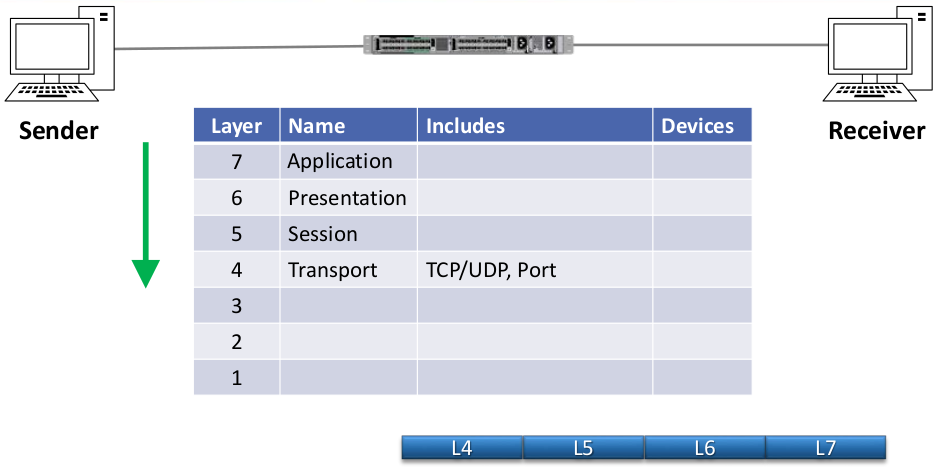
\includegraphics[width=\linewidth]{img/img05}
	\end{center}
\end{frame}

\begin{frame}{OSI Reference Model (Encapsulation)}
	\begin{center}
		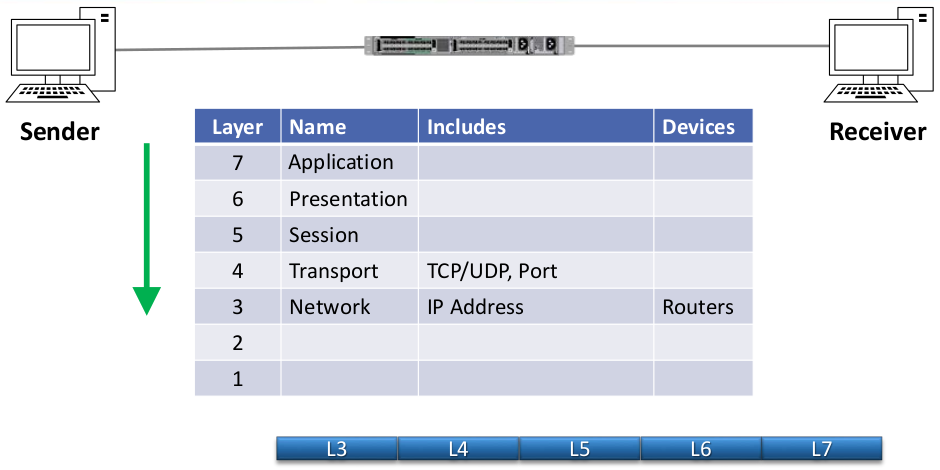
\includegraphics[width=\linewidth]{img/img06}
	\end{center}
\end{frame}

\begin{frame}
	\frametitle{The Domain Name System}
	\begin{itemize}
		\item The Domain Name System (DNS) resolves a Fully Qualified Domain Name (FQDN) such as www.cisco.com to an IP address.
		\item Enterprises will typically have an internal DNS server which can resolve the IP addresses of internal hosts.
		\item Hosts will send their DNS queries to this server.
		\item If the internal DNS server cannot resolve a query, it will forward the request out to public DNS servers on the Internet.
		\item DNS requests are sent using UDP port 53 (and can fail over to TCP).
	\end{itemize}
\end{frame}

\section{DNS on Cisco Routers}

\begin{frame}
	\frametitle{Router DNS Commands}
	\begin{itemize}
		\item DNS Client:
		\begin{itemize}
			\item[] \texttt{ip domain-lookup}
			\item[] \texttt{ip name-server 172.23.4.1}
			\item[] \texttt{ip domain-name flackboxA.lab} (primary domain name)
			\item[] \texttt{ip domain-list flackboxB.lab} (additional DNS suffixes to search)
		\end{itemize}
		\item Additional DNS Server Commands:
		\begin{itemize}
			\item[] \texttt{ip dns server}
			\item[] \texttt{ip host LinuxA 172.23.4.2}
		\end{itemize}
	\end{itemize}
\end{frame}

\section{ARP - Address Resolution Protocol}

\begin{frame}
	\frametitle{OSI Reference Model (Encapsulation)}
	\begin{center}
		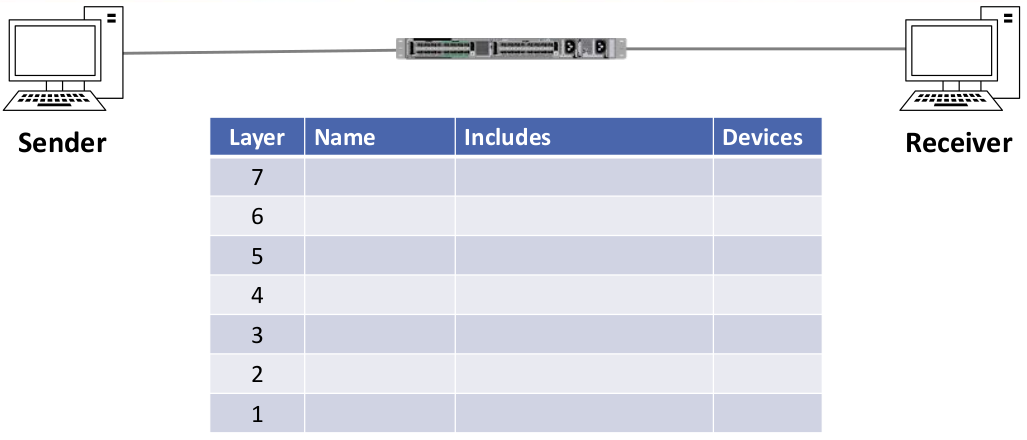
\includegraphics[width=\linewidth]{img/img01}
	\end{center}
\end{frame}

\begin{frame}{OSI Reference Model (Encapsulation)}
	\begin{center}
		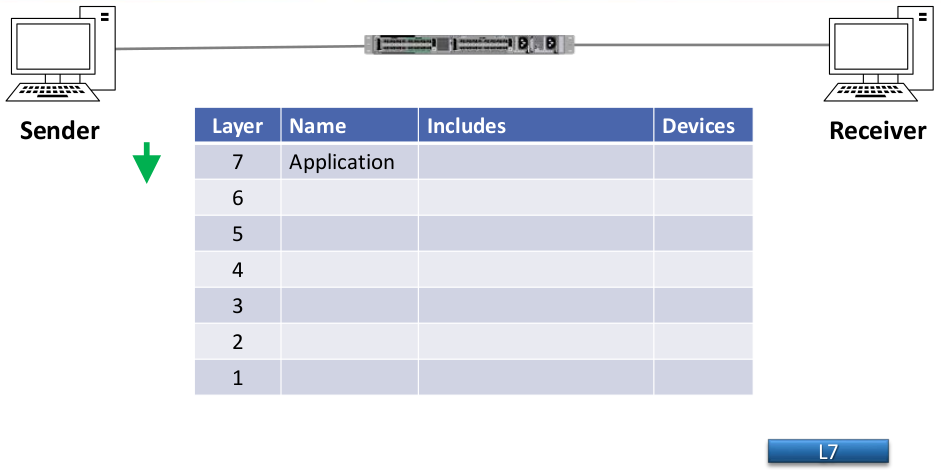
\includegraphics[width=\linewidth]{img/img02}
	\end{center}
\end{frame}

\begin{frame}{OSI Reference Model (Encapsulation)}
	\begin{center}
		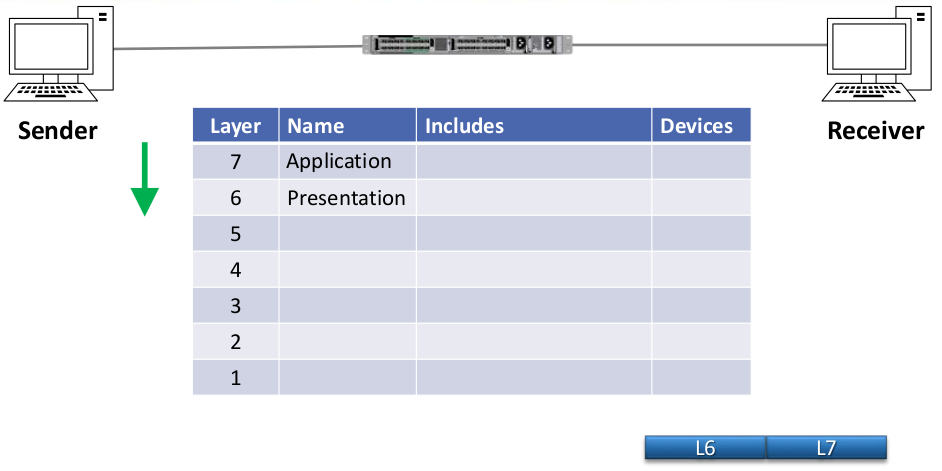
\includegraphics[width=\linewidth]{img/img03}
	\end{center}
\end{frame}

\begin{frame}{OSI Reference Model (Encapsulation)}
	\begin{center}
		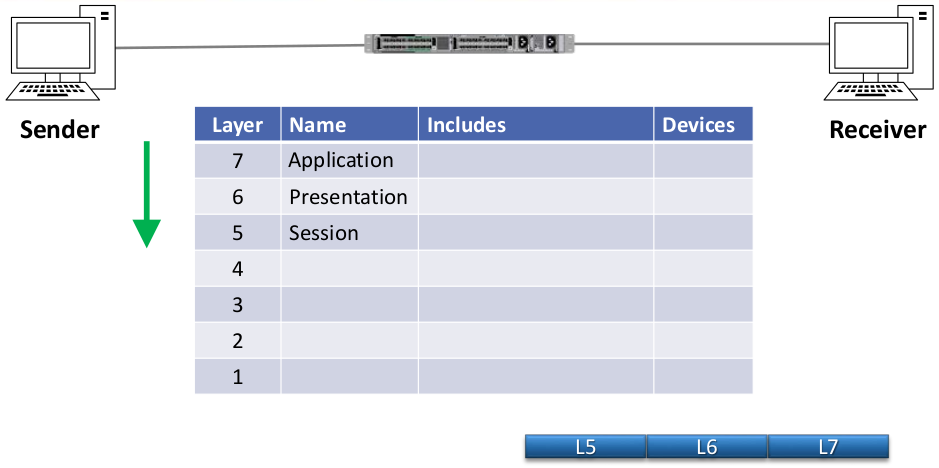
\includegraphics[width=\linewidth]{img/img04}
	\end{center}
\end{frame}

\begin{frame}{OSI Reference Model (Encapsulation)}
	\begin{center}
		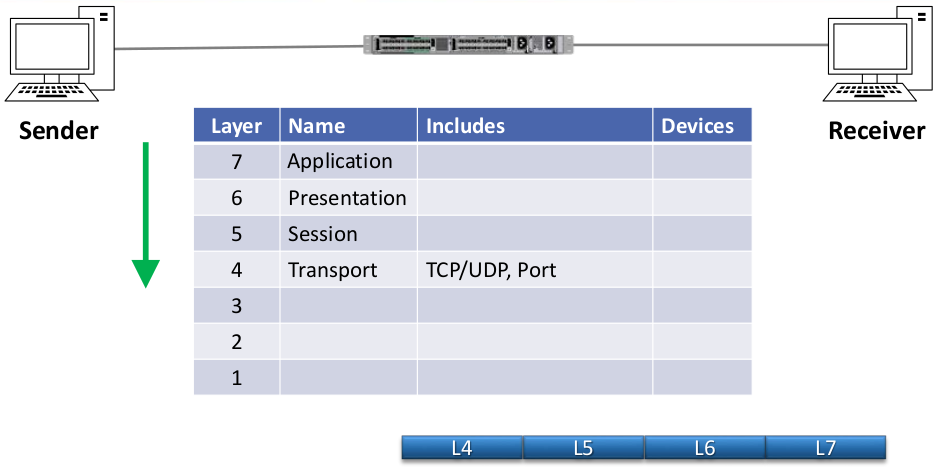
\includegraphics[width=\linewidth]{img/img05}
	\end{center}
\end{frame}

\begin{frame}{OSI Reference Model (Encapsulation)}
	\begin{center}
		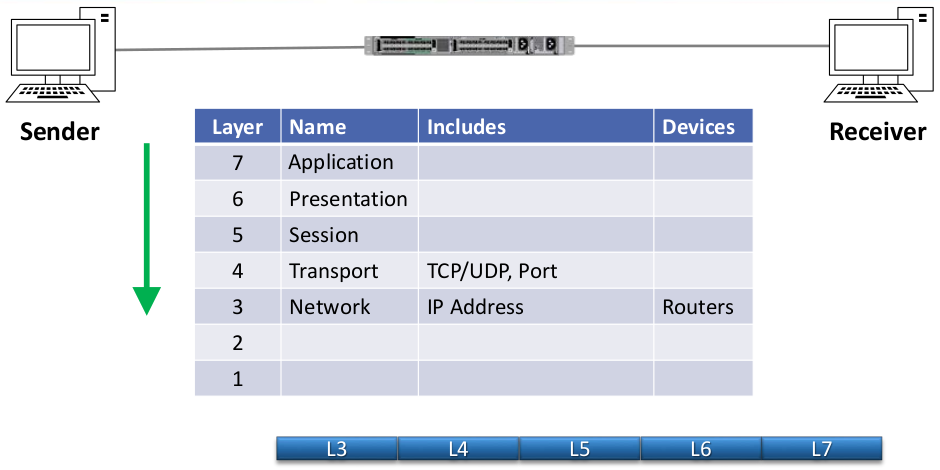
\includegraphics[width=\linewidth]{img/img06}
	\end{center}
\end{frame}

\begin{frame}{OSI Reference Model (Encapsulation)}
	\begin{center}
		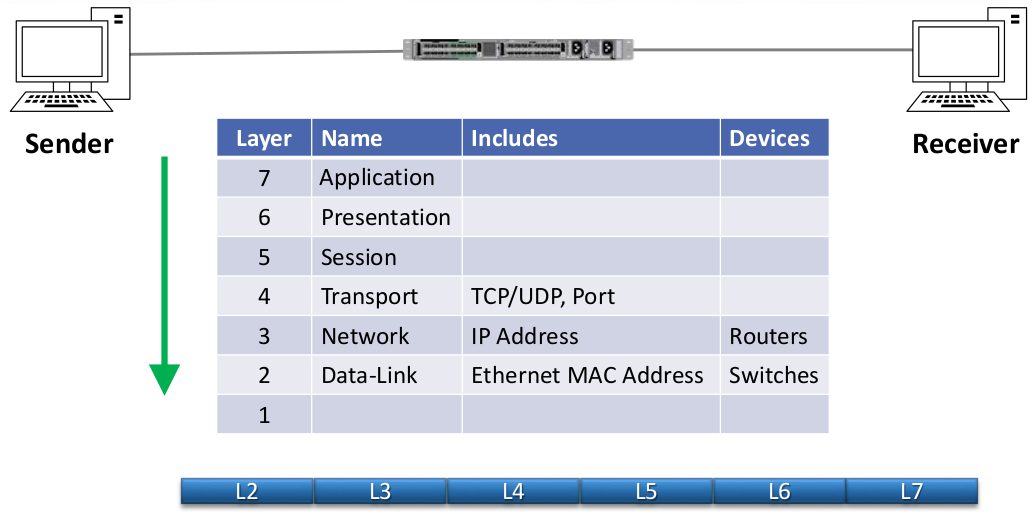
\includegraphics[width=\linewidth]{img/img07}
	\end{center}
\end{frame}

\begin{frame}
	\frametitle{IP to MAC Address Resolution}
	\begin{itemize}
		\item The sender needs to know the receiver’s IP address and MAC address to form the packet it’s going to send
		\item We can point the sender directly at the destination IP address or at a user friendly FQDN such as www.cisco.com
		\item DNS Domain Name System maintains a mapping of FQDNs to IP addresses
		\item ARP Address Resolution Protocol is used to map the IP address to MAC address
	\end{itemize}
\end{frame}

\begin{frame}
	\frametitle{ARP Address Resolution Protocol}
	\begin{center}
		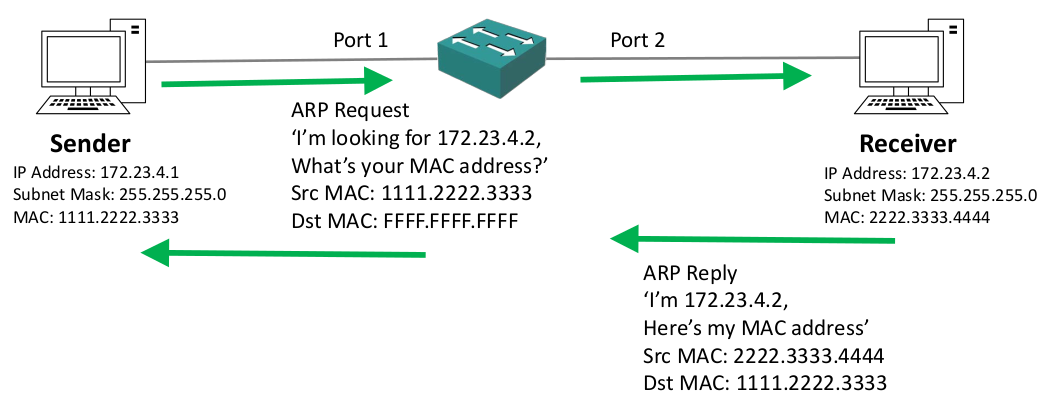
\includegraphics[width=\linewidth]{img/img08}
	\end{center}
\end{frame}

\begin{frame}
	\frametitle{Host ARP Commands}
	\begin{itemize}
		\item ARP replies are saved in a hosts ARP cache so it doesn’t need to send an ARP request every time it wants to communicate
		\item \textbf{Windows}
		\item[] View ARP cache: \texttt{arp -a}
		\item[] Clear ARP cache: \texttt{netsh interface ip delete} arpcache
		\item \textbf{Linux}
		\item[] View ARP cache: \texttt{arp -n}
		\item[] Clear ARP cache: \texttt{ip -s -s neigh flush all}
	\end{itemize}
\end{frame}

\section{ARP for Routed Traffic}

\begin{frame}
	\frametitle{Routed Traffic}
	\begin{itemize}
		\item When the sender and receiver are on different IP subnets, the traffic must be forwarded by a router
		\item In the following example, 172.23.4.1/24 wants to send a packet to 192.168.10.1/24
	\end{itemize}
\end{frame}

\begin{frame}
	\frametitle{Routing Traffic}
	\begin{center}
		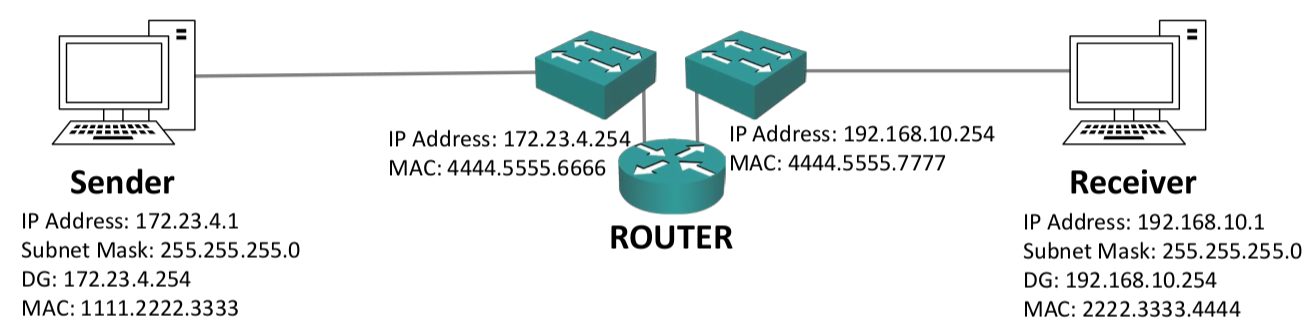
\includegraphics[width=\linewidth]{img/img09}
	\end{center}
\end{frame}

\begin{frame}{Routing Traffic}
	\begin{center}
		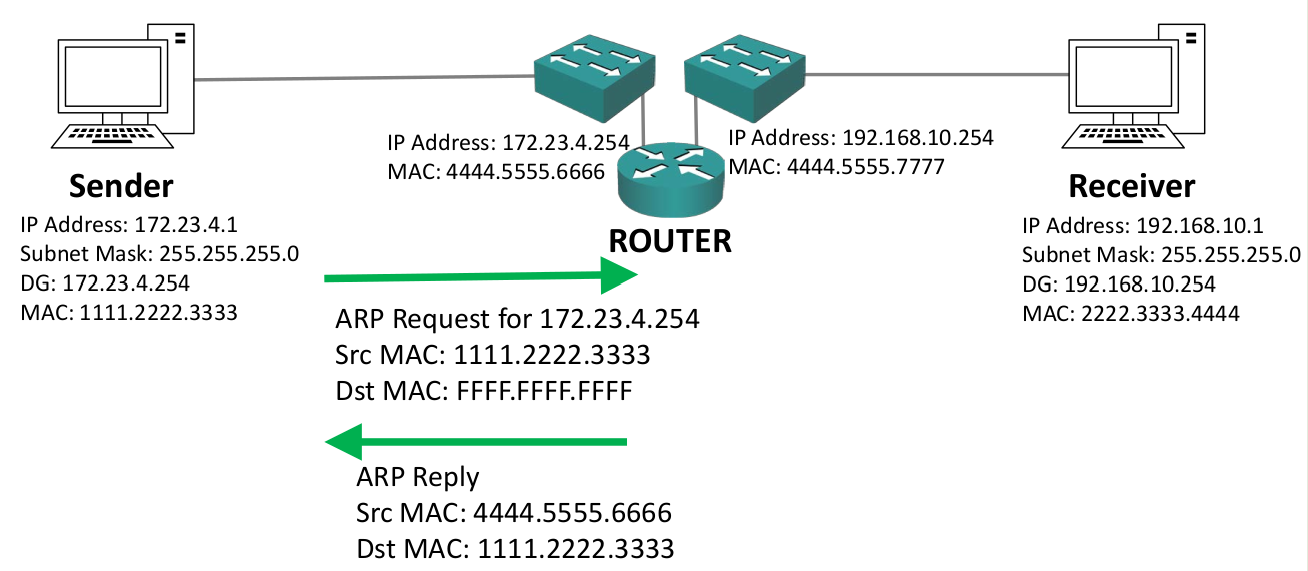
\includegraphics[width=\linewidth]{img/img10}
	\end{center}
\end{frame}

\begin{frame}{Routing Traffic}
	\begin{center}
		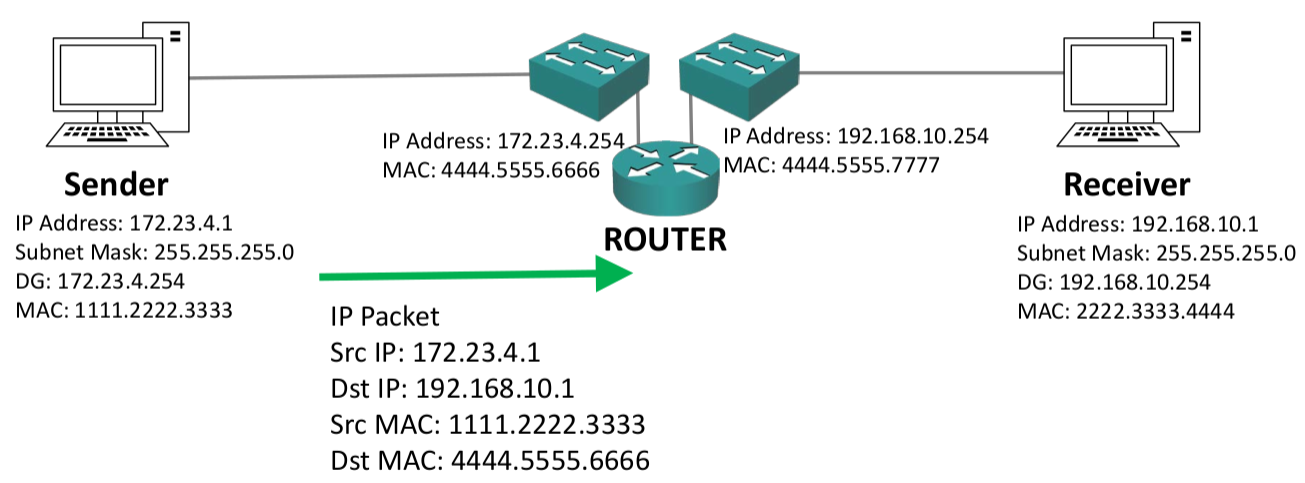
\includegraphics[width=\linewidth]{img/img11}
	\end{center}
\end{frame}

\begin{frame}{Routing Traffic}
	\begin{center}
		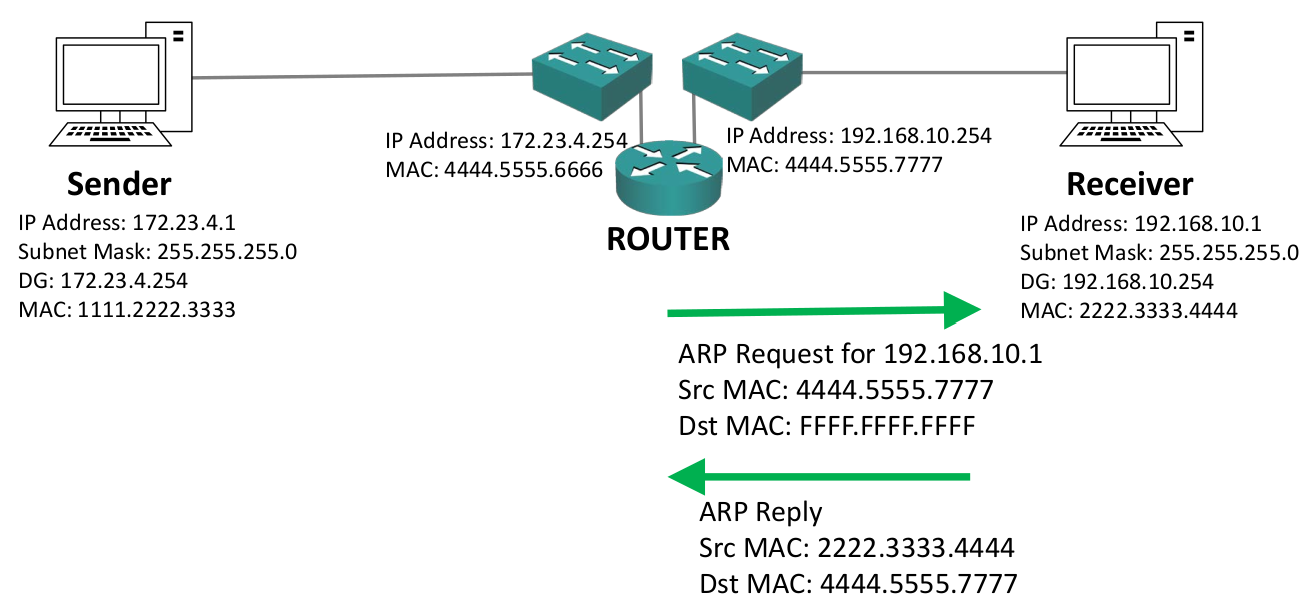
\includegraphics[width=\linewidth]{img/img12}
	\end{center}
\end{frame}

\begin{frame}{Routing Traffic}
	\begin{center}
		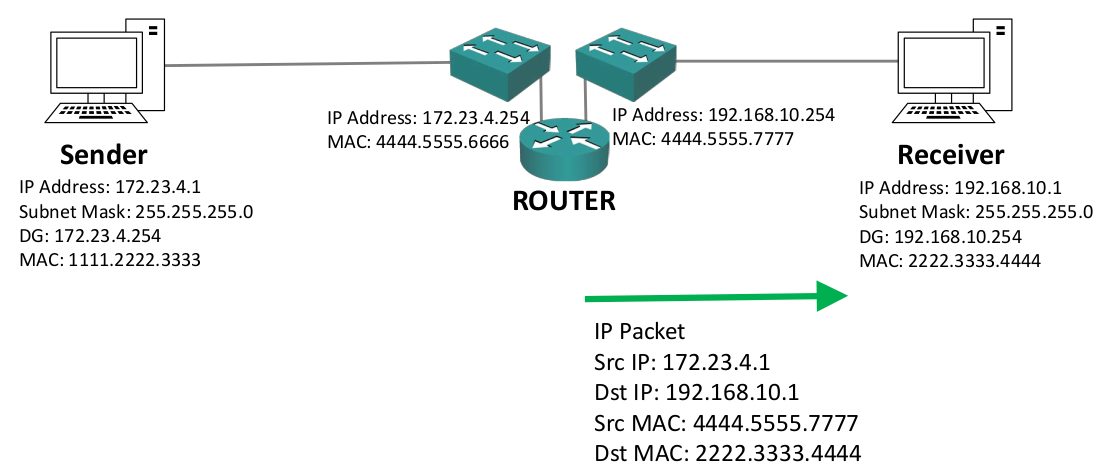
\includegraphics[width=\linewidth]{img/img13}
	\end{center}
\end{frame}

\begin{frame}
	\frametitle{Router ARP Commands}
	\begin{itemize}
		\item View ARP cache: \texttt{show arp}
		\item Clear ARP cache: \texttt{clear arp-cache}
	\end{itemize}
\end{frame}

\section{The Life of a Packet}

\begin{frame}
	\frametitle{The Life of a Packet}
	\begin{center}
		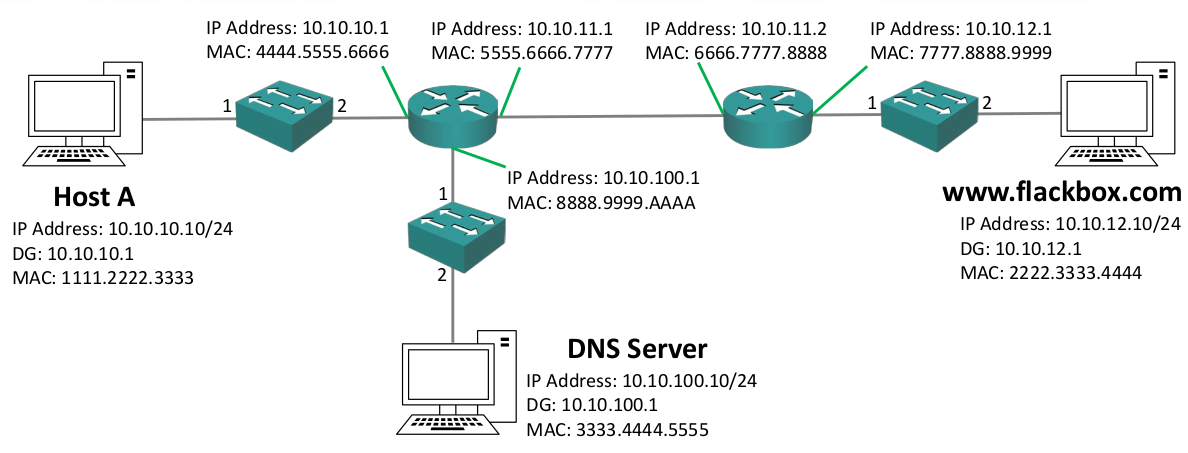
\includegraphics[width=\linewidth]{img/img14}
	\end{center}
\end{frame}

\begin{frame}
	\frametitle{OSI Reference Model (Encapsulation)}
	\begin{center}
		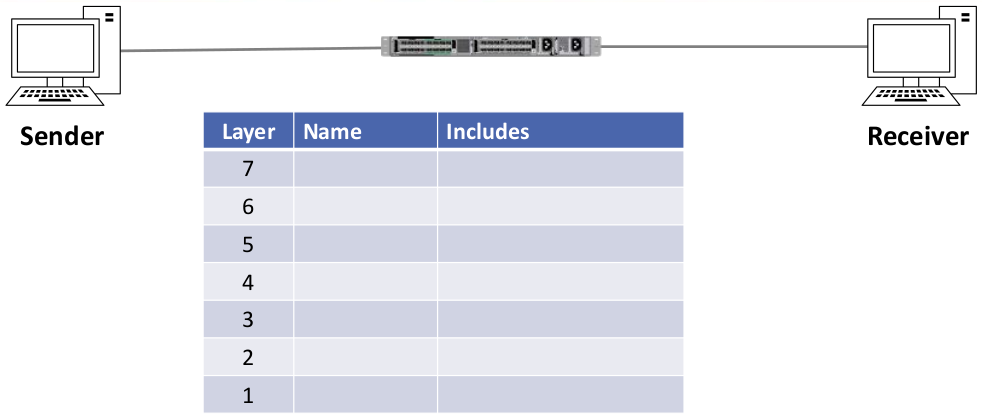
\includegraphics[width=\linewidth]{img/img65}
	\end{center}
\end{frame}

\begin{frame}{OSI Reference Model (Encapsulation)}
	\begin{center}
		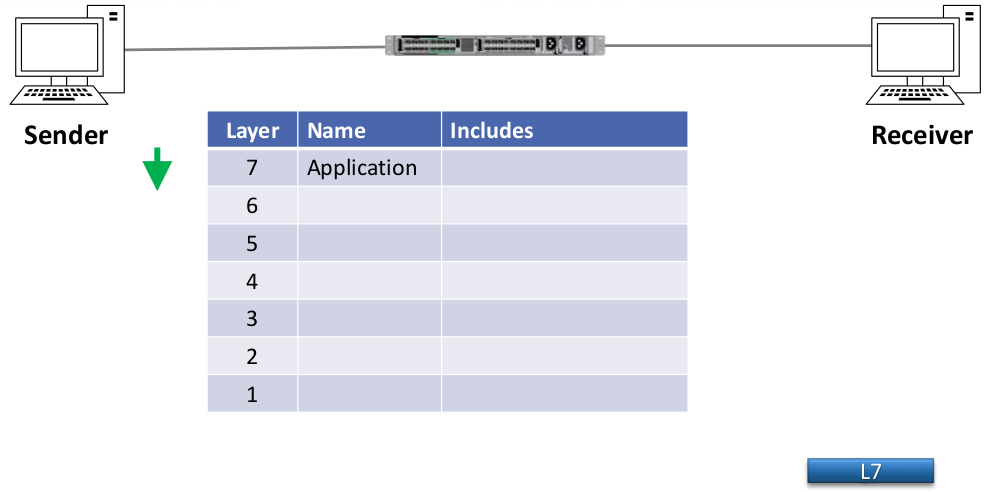
\includegraphics[width=\linewidth]{img/img66}
	\end{center}
\end{frame}

\begin{frame}{OSI Reference Model (Encapsulation)}
	\begin{center}
		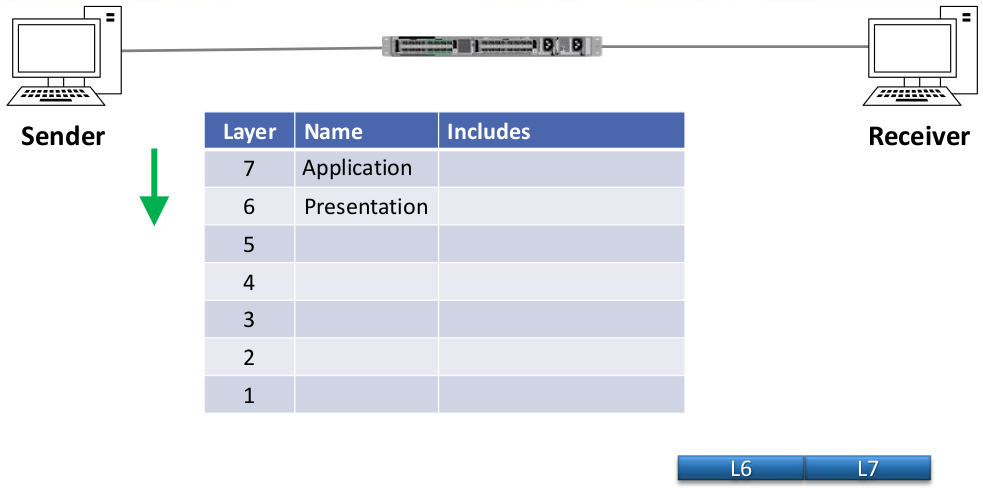
\includegraphics[width=\linewidth]{img/img67}
	\end{center}
\end{frame}

\begin{frame}{OSI Reference Model (Encapsulation)}
	\begin{center}
		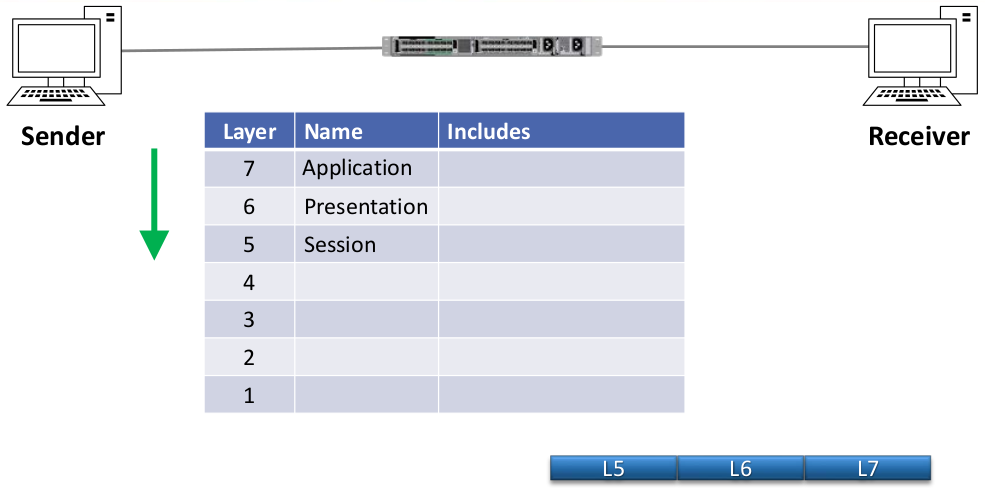
\includegraphics[width=\linewidth]{img/img68}
	\end{center}
\end{frame}

\begin{frame}{OSI Reference Model (Encapsulation)}
	\begin{center}
		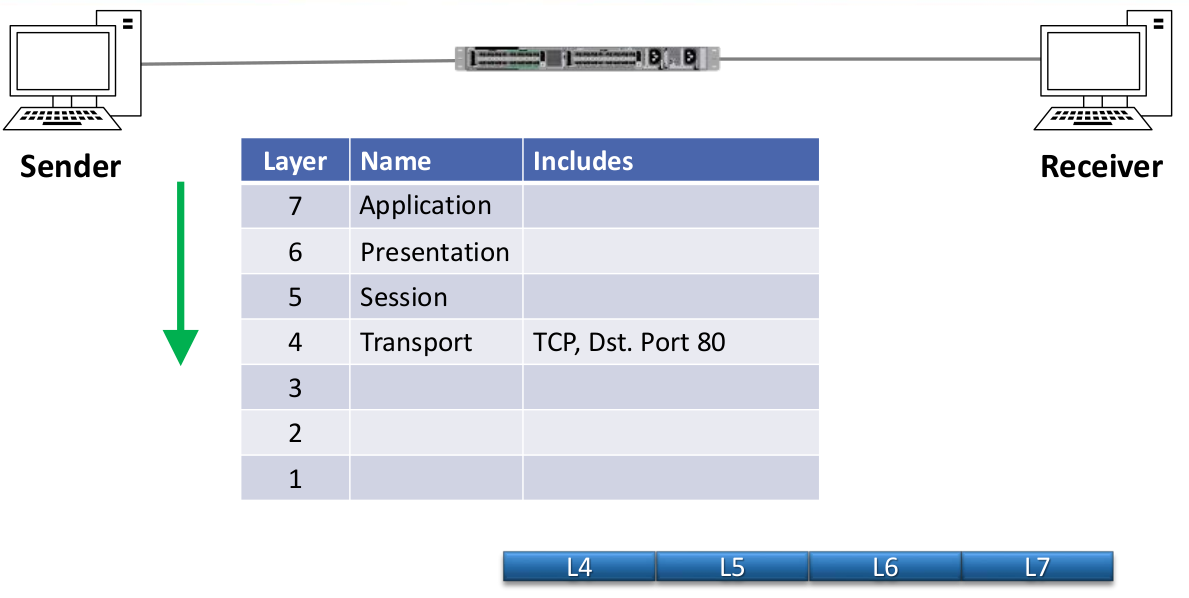
\includegraphics[width=\linewidth]{img/img15}
	\end{center}
\end{frame}


\begin{frame}{OSI Reference Model (Encapsulation)}
	\begin{center}
		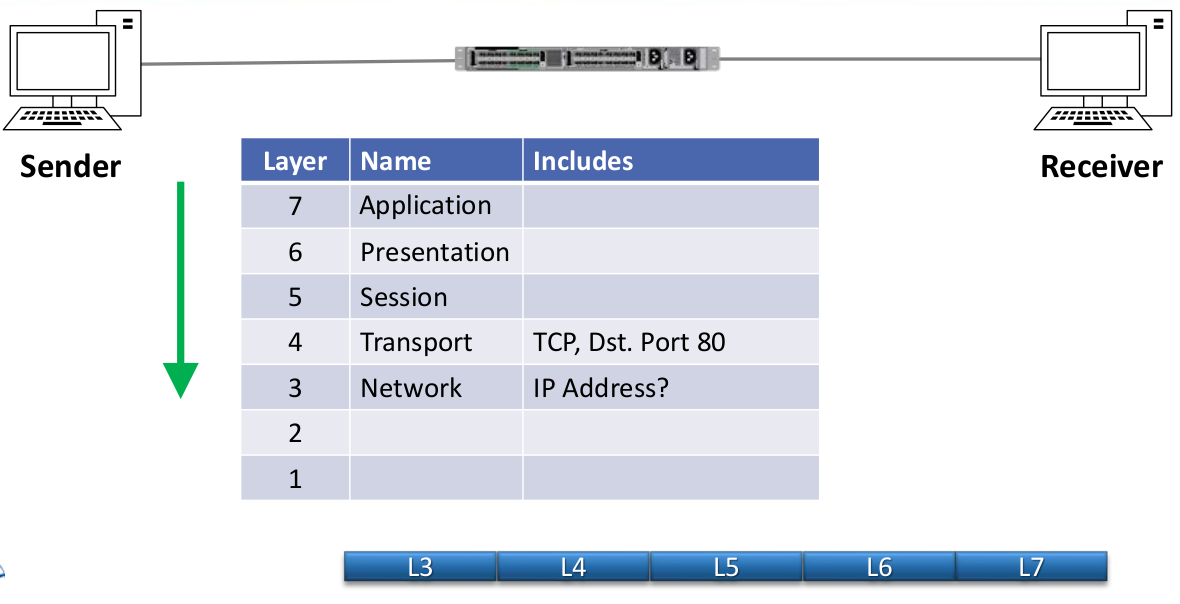
\includegraphics[width=\linewidth]{img/img16}
	\end{center}
\end{frame}

\begin{frame}
	\frametitle{The Life of a Packet}
	\begin{itemize}
		\item Host A (10.10.10.10/24) wants to send a packet to the FQDN www.flackbox.com, but it doesn’t know the destination IP address
		\item It will hold the packet and send a DNS request to its DNS server at 10.10.100.10
		\item Host A compares its IP address and subnet mask to the destination address of the DNS server and sees it is on a different subnet, so the DNS request needs to be sent via its default gateway
		\item Host A will hold the DNS request and send a broadcast ARP request for its default gateway at 10.10.10.1
	\end{itemize}
\end{frame}

\begin{frame}{The Life of a Packet}
	\begin{center}
		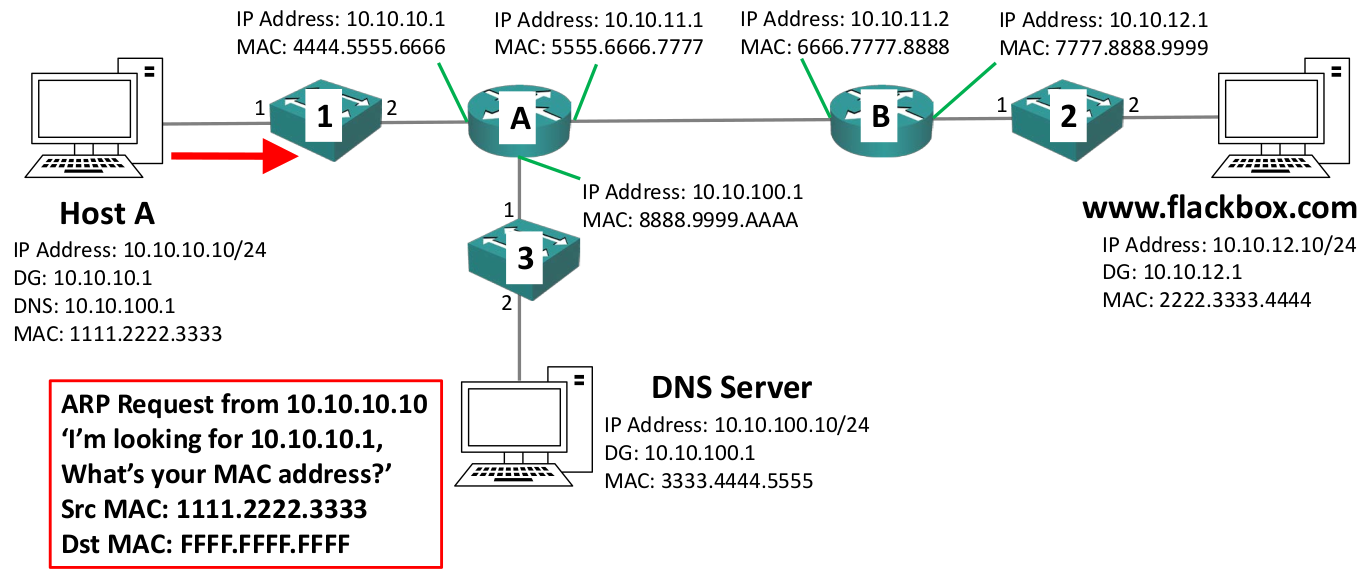
\includegraphics[width=\linewidth]{img/img17}
	\end{center}
\end{frame}

\begin{frame}{The Life of a Packet}
	\begin{itemize}
		\item The ARP request will be received by Switch 1
		\item Switch 1 will add an entry in its MAC address table mapping Host A’s MAC address 1111.2222.3333 to Port 1
		\item Switch 1 will flood the broadcast traffic out all ports apart from the one it was received on
	\end{itemize}
\end{frame}

\begin{frame}{The Life of a Packet}
	\begin{center}
		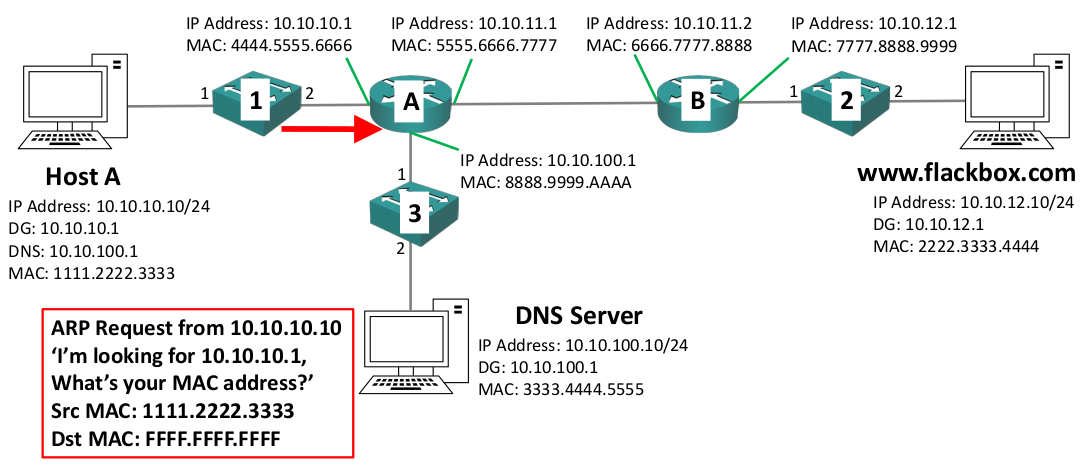
\includegraphics[width=\linewidth]{img/img18}
	\end{center}
\end{frame}

\begin{frame}{The Life of a Packet}
	\begin{itemize}
		\item The ARP request will hit Router A’s interface 10.10.10.1
		\item Router A will process the ARP request and see it is for itself
		\item Router A will send a unicast ARP reply to Host A
		\item Router A will add an entry for Host A mapping IP address 10.10.10.10 to MAC address 1111.2222.3333 to its ARP cache
	\end{itemize}
\end{frame}

\begin{frame}{The Life of a Packet}
	\begin{center}
		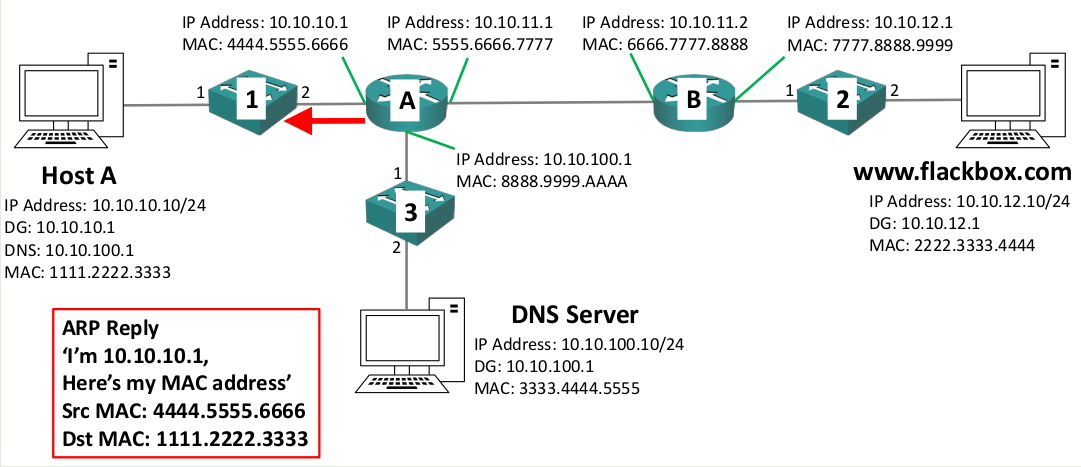
\includegraphics[width=\linewidth]{img/img19}
	\end{center}
\end{frame}

\begin{frame}{The Life of a Packet}
	\begin{itemize}
		\item Switch 1 will add an entry in its MAC address table mapping Router A’s MAC address 4444.5555.6666 to Port 2
		\item Switch 1 will send the ARP reply out only Port 1 which Host A is plugged into (which it already has in its MAC address table)
	\end{itemize}
\end{frame}

\begin{frame}{The Life of a Packet}
	\begin{center}
		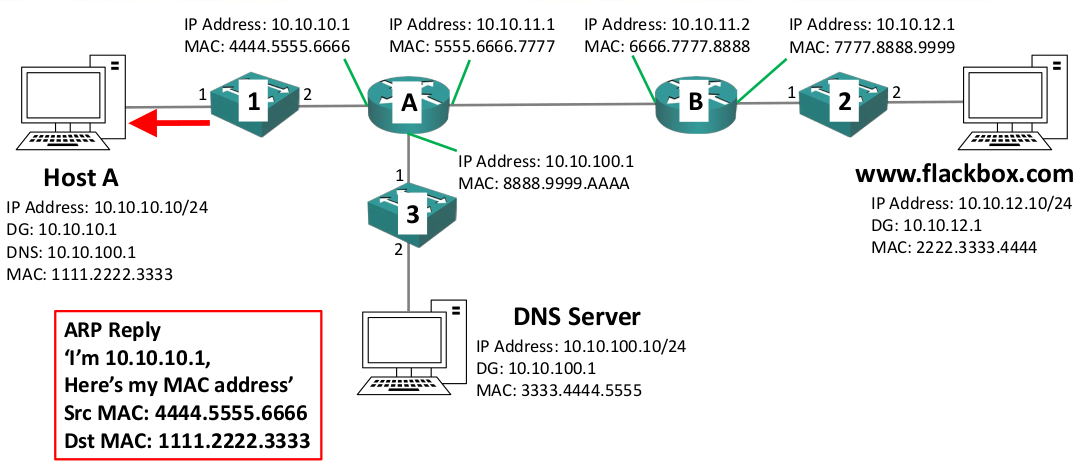
\includegraphics[width=\linewidth]{img/img20}
	\end{center}
\end{frame}

\begin{frame}{The Life of a Packet}
	\begin{itemize}
		\item Host A will add an entry for Router A mapping IP address 10.10.10.1 to MAC address 4444.5555.6666 to its ARP cache
		\item It will use this whenever it needs to send traffic to another IP subnet
		\item Host A will send the DNS request for www.flackbox.com
	\end{itemize}
\end{frame}

\begin{frame}{The Life of a Packet}
	\begin{center}
		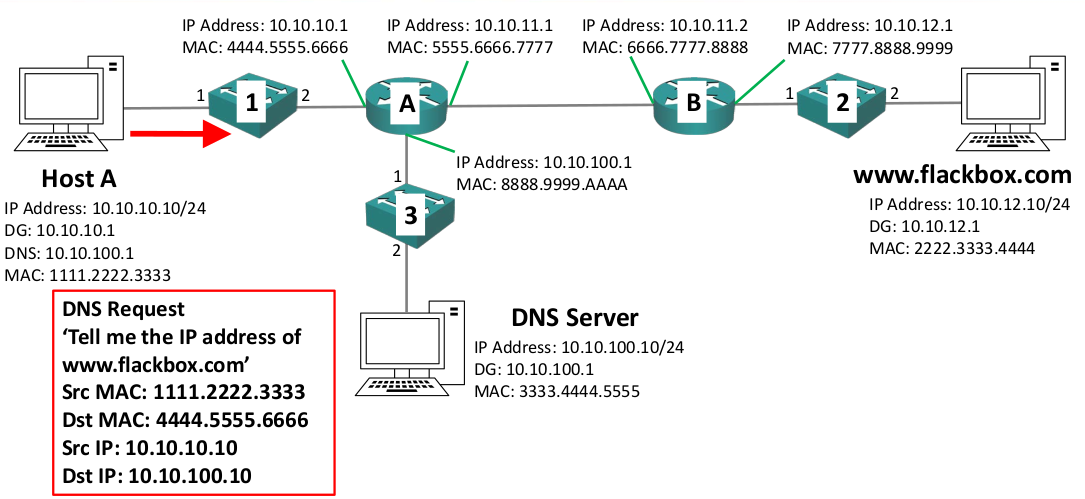
\includegraphics[width=\linewidth]{img/img21}
	\end{center}
\end{frame}

\begin{frame}{The Life of a Packet}
	\begin{itemize}
		\item Switch 1 will send the DNS request out only Port 2 which Router A is plugged into (which it already has in its MAC address table)
	\end{itemize}
\end{frame}

\begin{frame}{The Life of a Packet}
	\begin{center}
		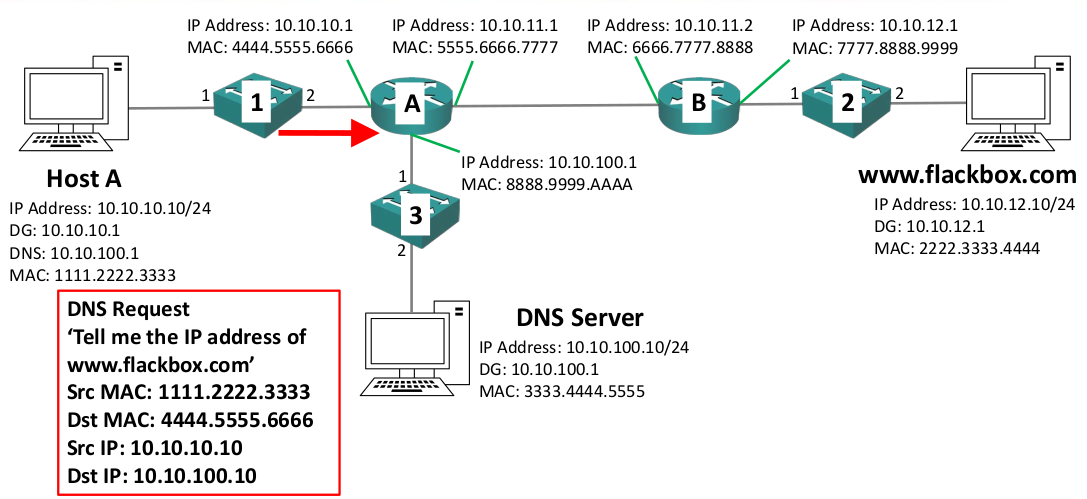
\includegraphics[width=\linewidth]{img/img22}
	\end{center}
\end{frame}

\begin{frame}{The Life of a Packet}
	\begin{itemize}
		\item Router A will receive the DNS request packet and see that the destination IP address is 10.10.100.10
		\item Router A has an interface in the subnet 10.10.100.0/24, so it knows the destination should be available out that port
		\item It doesn’t know the MAC address of 10.10.100.10 so it will hold the DNS request packet and send an ARP request out of the 10.10.100.1
		interface
	\end{itemize}
\end{frame}

\begin{frame}{The Life of a Packet}
	\begin{center}
		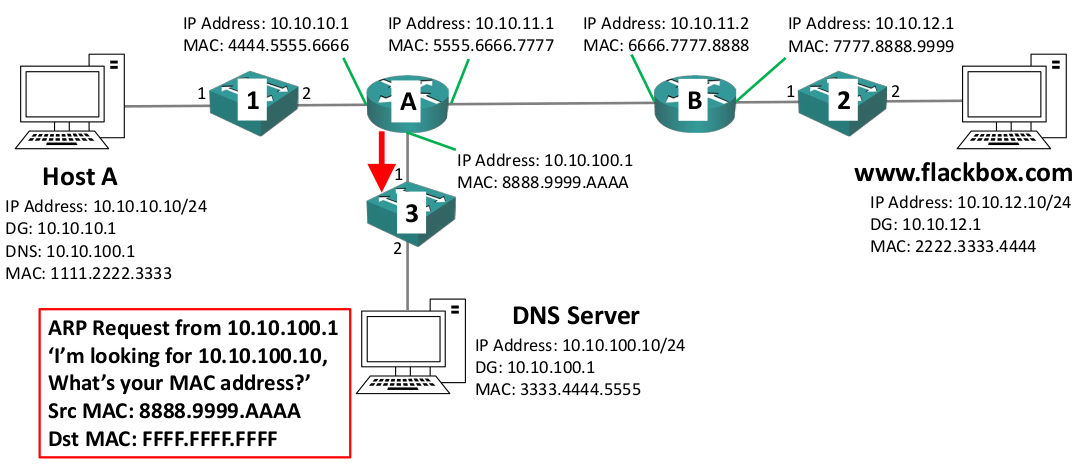
\includegraphics[width=\linewidth]{img/img23}
	\end{center}
\end{frame}

\begin{frame}{The Life of a Packet}
	\begin{itemize}
		\item The ARP request will be received by Switch 3 
		\item Switch 3 will add an entry in its MAC address table mapping Router A’s MAC address 8888.9999.AAAA to Port 1
		\item Switch 3 will flood the broadcast traffic out all ports apart from the one it was received on
	\end{itemize}
\end{frame}

\begin{frame}{The Life of a Packet}
	\begin{center}
		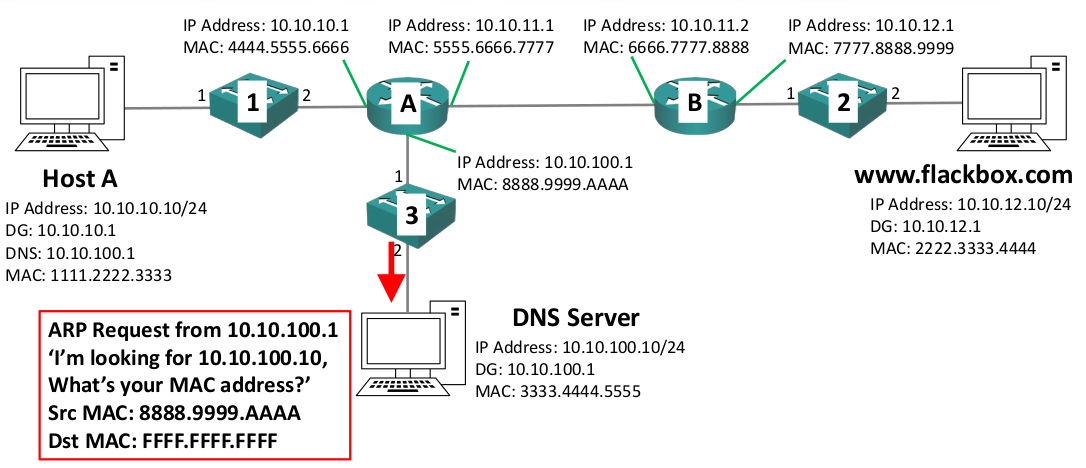
\includegraphics[width=\linewidth]{img/img24}
	\end{center}
\end{frame}

\begin{frame}{The Life of a Packet}
	\begin{itemize}
		\item The ARP request will hit the DNS Server’s interface 10.10.100.10
		\item The DNS Server will process the ARP request and see it is for itself
		\item The DNS Server will send a unicast ARP reply to Router A
		\item The DNS Server will add an entry for Router A mapping IP address 10.10.100.1 to MAC address 8888.9999.AAAA to its ARP cache
		\item It will use this whenever it needs to send traffic to another IP subnet
	\end{itemize}
\end{frame}

\begin{frame}{The Life of a Packet}
	\begin{center}
		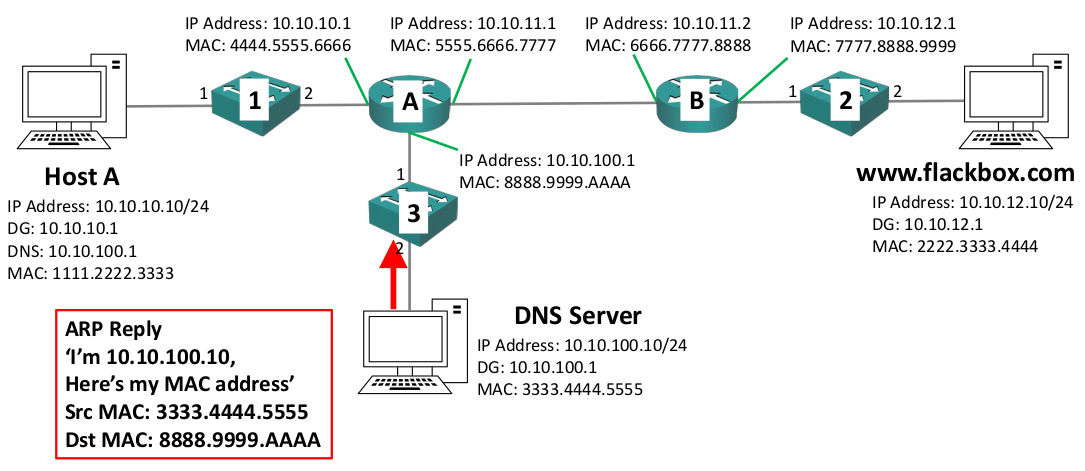
\includegraphics[width=\linewidth]{img/img25}
	\end{center}
\end{frame}

\begin{frame}{The Life of a Packet}
	\begin{itemize}
		\item Switch 3 will add an entry in its MAC address table mapping the DNS Server’s MAC address 3333.4444.5555 to Port 2
		\item Switch 3 will send the ARP reply out only Port 1 which Router A is plugged into (which it already has in its MAC address table)
	\end{itemize}
\end{frame}

\begin{frame}{The Life of a Packet}
	\begin{center}
		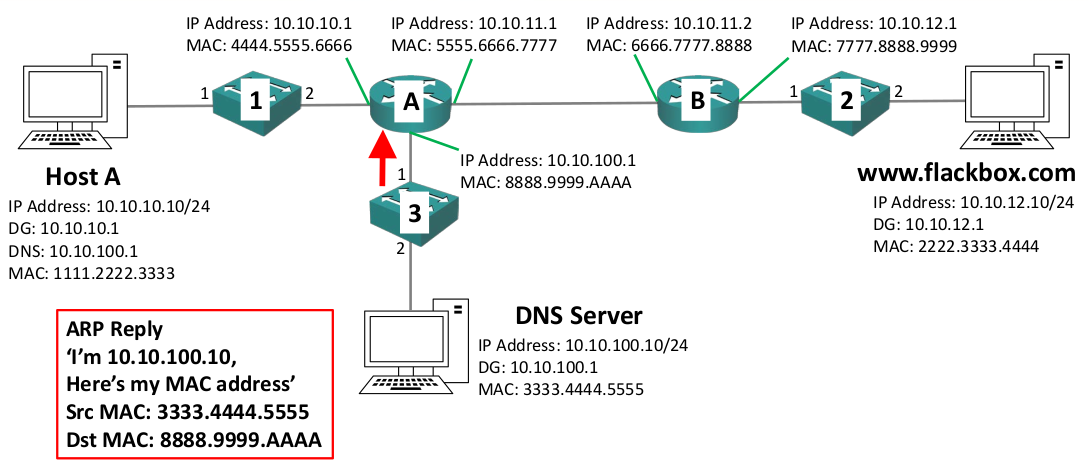
\includegraphics[width=\linewidth]{img/img26}
	\end{center}
\end{frame}

\begin{frame}{The Life of a Packet}
	\begin{itemize}
		\item Router A will add an entry for the DNS Server mapping IP address 10.10.100.10 to MAC address 3333.4444.5555 to its ARP cache
		\item Router A will send the DNS request it was holding to the DNS Server
	\end{itemize}
\end{frame}

\begin{frame}{The Life of a Packet}
	\begin{itemize}
		\item \textbf{The source and destination MAC addresses of a packet are updated hop by hop, the source and destination IP addresses always remain unchanged end to end}
		\item The source and destination MAC addresses will be updated to come from Router A and go to the DNS Server
		\item The source and destination IP addresses are still Host A 10.10.10.10 and the DNS Server 10.10.100.10
	\end{itemize}
\end{frame}

\begin{frame}{The Life of a Packet}
	\begin{center}
		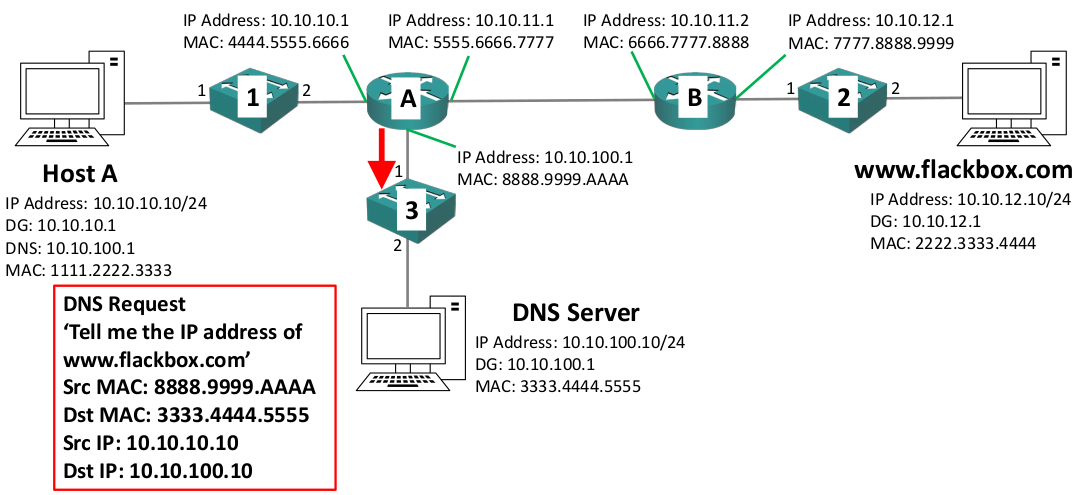
\includegraphics[width=\linewidth]{img/img27}
	\end{center}
\end{frame}

\begin{frame}{The Life of a Packet}
	\begin{itemize}
		\item Switch 3 will send the DNS request out only Port 2 which the DNS Server is plugged into (which it already has in its MAC address table)
	\end{itemize}
\end{frame}

\begin{frame}{The Life of a Packet}
	\begin{center}
		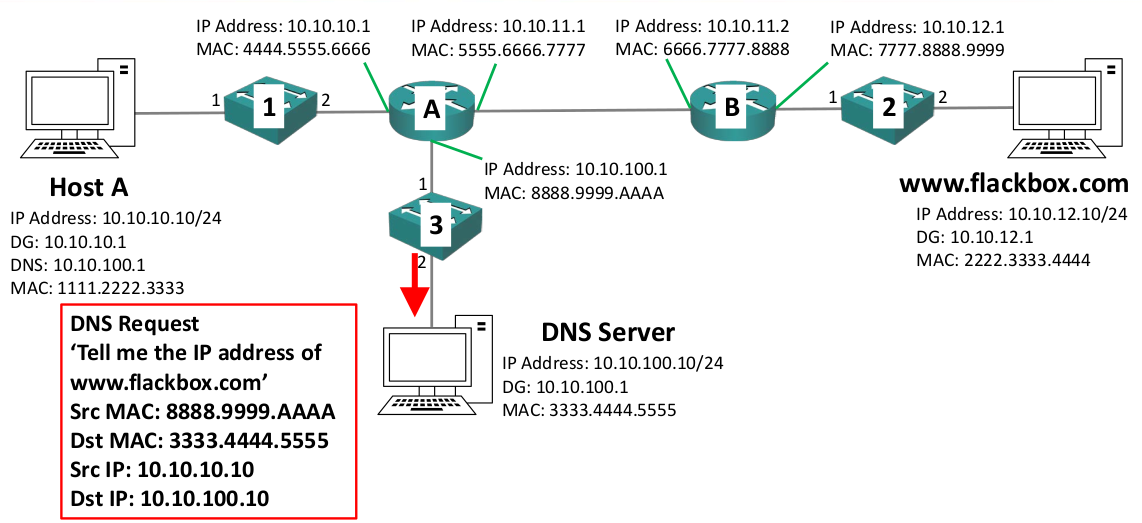
\includegraphics[width=\linewidth]{img/img28}
	\end{center}
\end{frame}

\begin{frame}{The Life of a Packet}
	\begin{itemize}
		\item The DNS Server will receive the DNS request packet and see that the
		destination is itself
	\end{itemize}
\end{frame}

\begin{frame}
	\frametitle{OSI Reference Model\\(De-encapsulation)}
	\begin{center}
		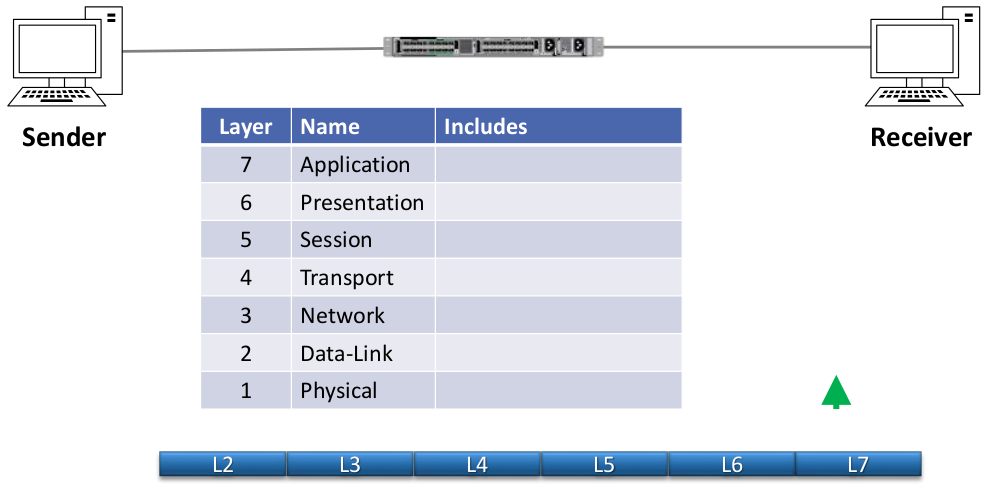
\includegraphics[width=\linewidth]{img/img29}
	\end{center}
\end{frame}

\begin{frame}{OSI Reference Model\\(De-encapsulation)}
	\begin{center}
		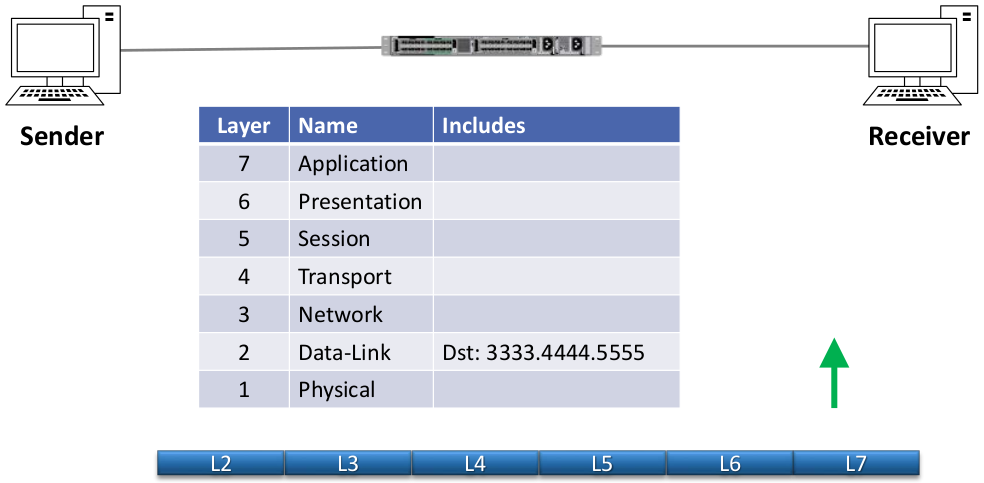
\includegraphics[width=\linewidth]{img/img30}
	\end{center}
\end{frame}

\begin{frame}{OSI Reference Model\\(De-encapsulation)}
	\begin{center}
		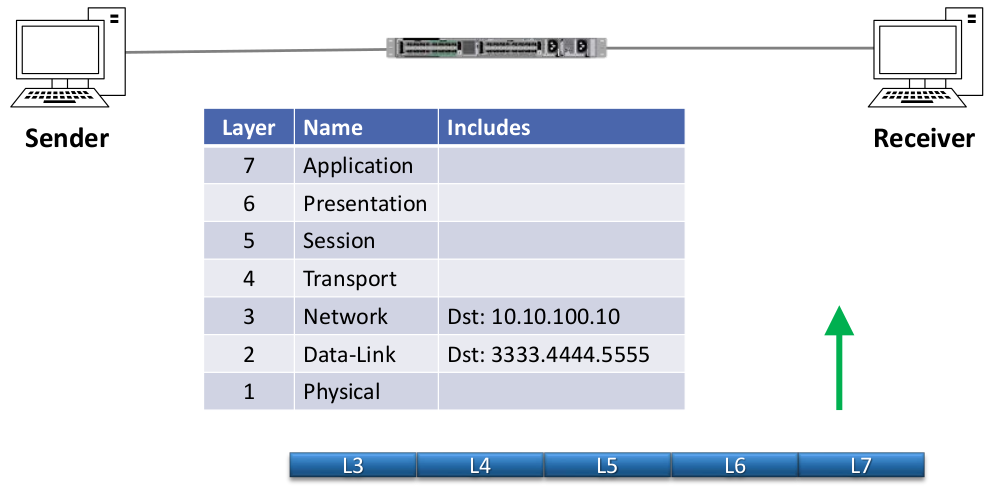
\includegraphics[width=\linewidth]{img/img31}
	\end{center}
\end{frame}

\begin{frame}{OSI Reference Model\\(De-encapsulation)}
	\begin{center}
		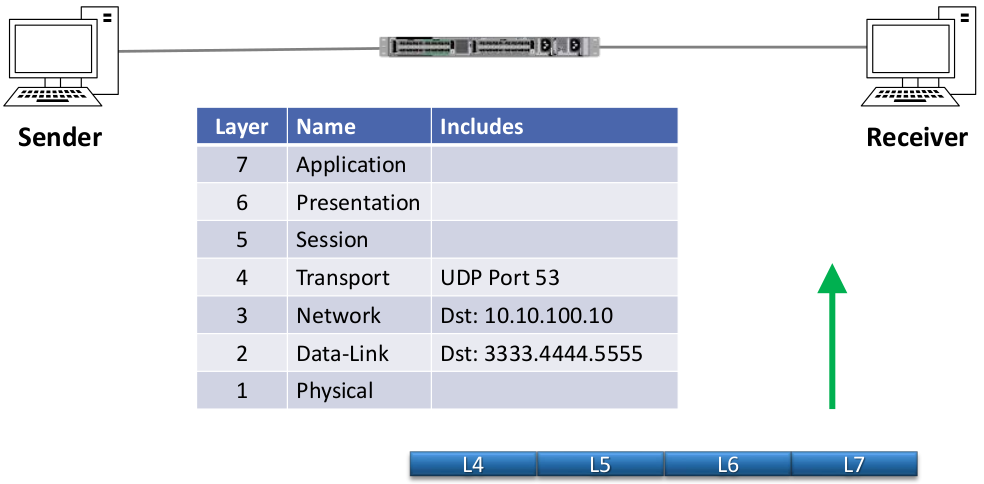
\includegraphics[width=\linewidth]{img/img32}
	\end{center}
\end{frame}

\begin{frame}{OSI Reference Model\\(De-encapsulation)}
	\begin{center}
		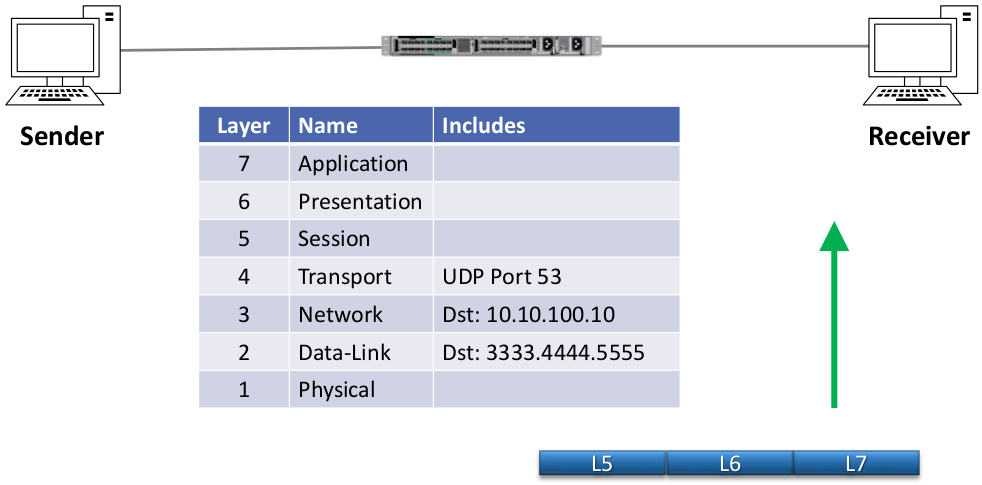
\includegraphics[width=\linewidth]{img/img33}
	\end{center}
\end{frame}

\begin{frame}{OSI Reference Model\\(De-encapsulation)}
	\begin{center}
		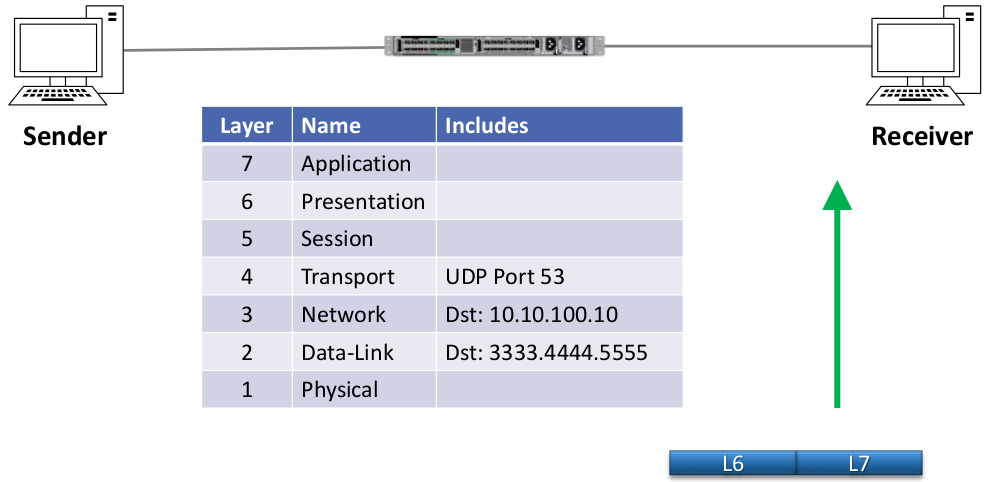
\includegraphics[width=\linewidth]{img/img34}
	\end{center}
\end{frame}

\begin{frame}{OSI Reference Model\\(De-encapsulation)}
	\begin{center}
		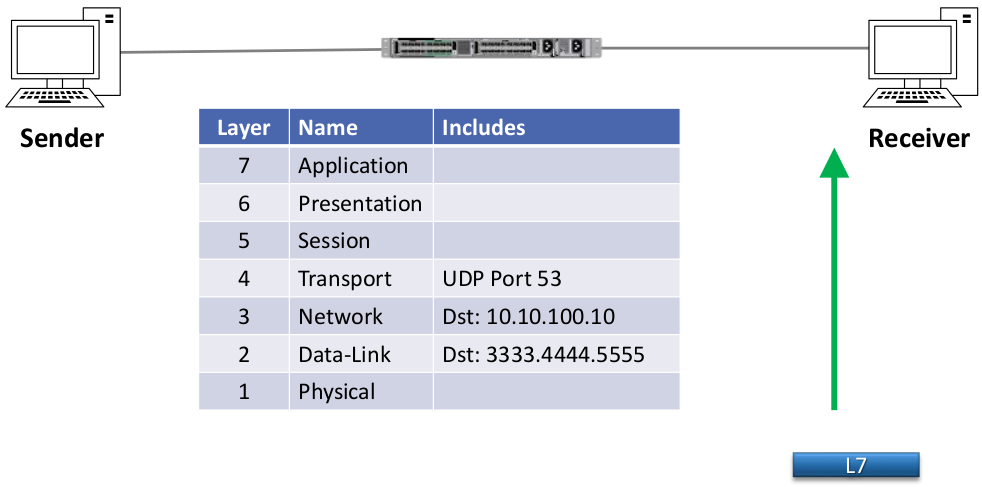
\includegraphics[width=\linewidth]{img/img35}
	\end{center}
\end{frame}

\begin{frame}
	\frametitle{The Life of a Packet}
	\begin{itemize}
		\item The DNS Server will look in its DNS database and see an Address record for www.flackbox.com at 10.10.12.10
		\item It will send this information to Host A in a DNS response
		\item It knows to send the response to 10.10.10.10 from the source IP address in the DNS request
		\item It knows to send it via Router A because the destination is in another subnet
		\item It already has Router A’s MAC address in its ARP cache
	\end{itemize}
\end{frame}

\begin{frame}{The Life of a Packet}
	\begin{center}
		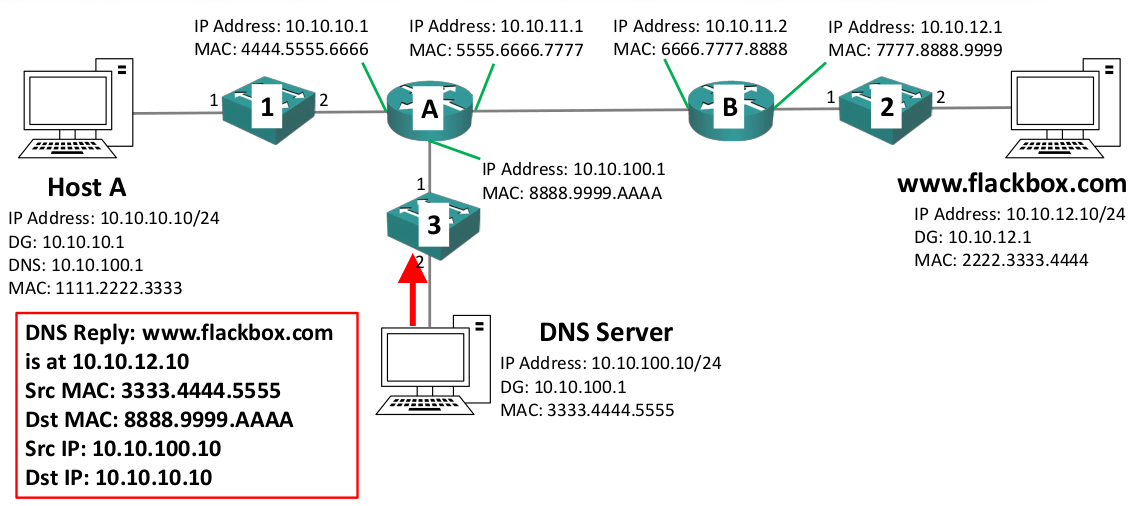
\includegraphics[width=\linewidth]{img/img36}
	\end{center}
\end{frame}

\begin{frame}{The Life of a Packet}
	\begin{itemize}
		\item Switch 3 will receive the DNS response and send it out only Port 1 which Router A is plugged into (which it already has in its MAC address
		table)
	\end{itemize}
\end{frame}

\begin{frame}{The Life of a Packet}
	\begin{center}
		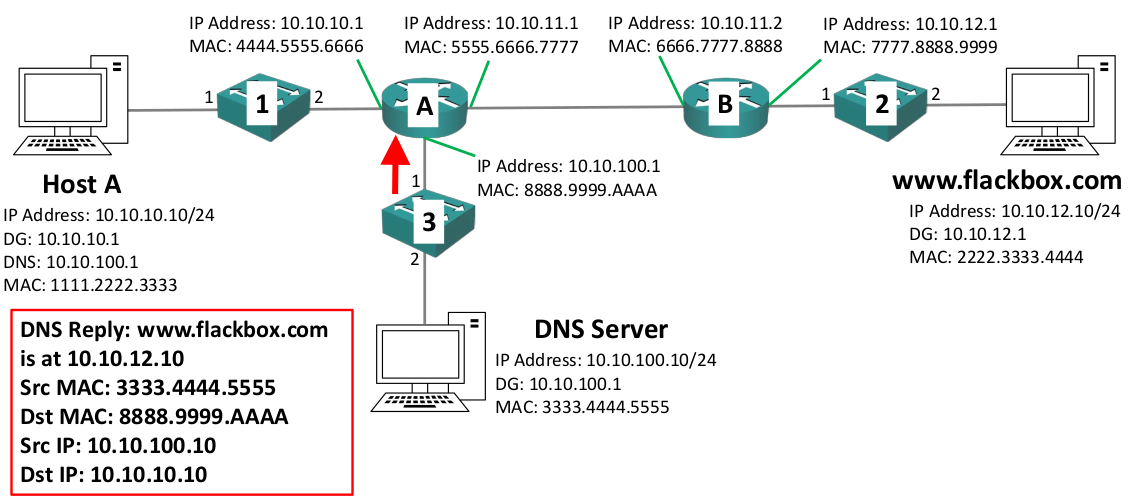
\includegraphics[width=\linewidth]{img/img37}
	\end{center}
\end{frame}

\begin{frame}{The Life of a Packet}
	\begin{itemize}
		\item Router A will receive the DNS response packet and see that the destination IP address is 10.10.10.10
		\item Router A has an interface in the subnet 10.10.10.0/24, so it knows the destination is available out that port
		\item Router A already has the MAC address for 10.10.10.10 in its ARP cache
	\end{itemize}
\end{frame}

\begin{frame}{The Life of a Packet}
	\begin{center}
		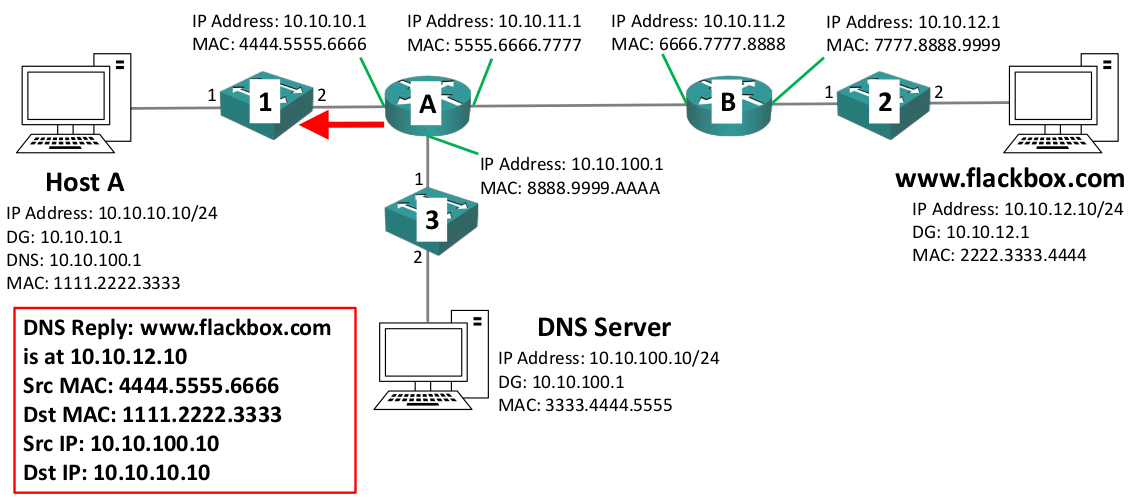
\includegraphics[width=\linewidth]{img/img38}
	\end{center}
\end{frame}

\begin{frame}{The Life of a Packet}
	\begin{itemize}
		\item Switch 1 will receive the DNS response and send it out only Port 1 which Host A is plugged into (which it already has in its MAC address
		table)
	\end{itemize}
\end{frame}

\begin{frame}{The Life of a Packet}
	\begin{center}
		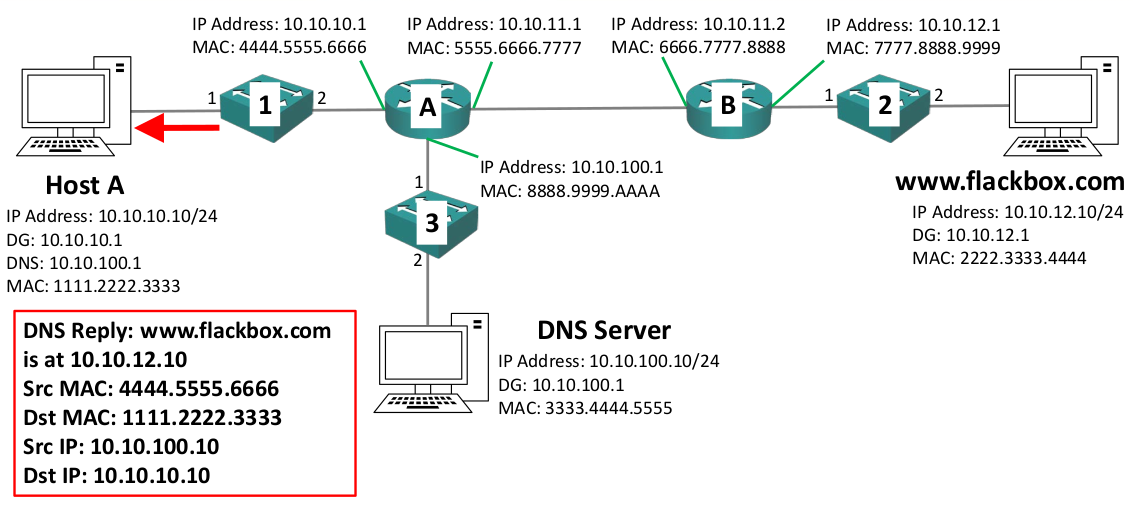
\includegraphics[width=\linewidth]{img/img39}
	\end{center}
\end{frame}

\begin{frame}{The Life of a Packet}
	\begin{itemize}
		\item Host A learns that www.flackbox.com is available at 10.10.12.10
		\item It can now update the packet it was waiting to send to www.flackbox.com with that destination IP address
		\item Host A sees that www.flackbox.com is not on its own subnet so it knows any packets it sends there must go via its default gateway
	\end{itemize}
\end{frame}

\begin{frame}
	\frametitle{OSI Reference Model (Encapsulation)}
	\begin{center}
		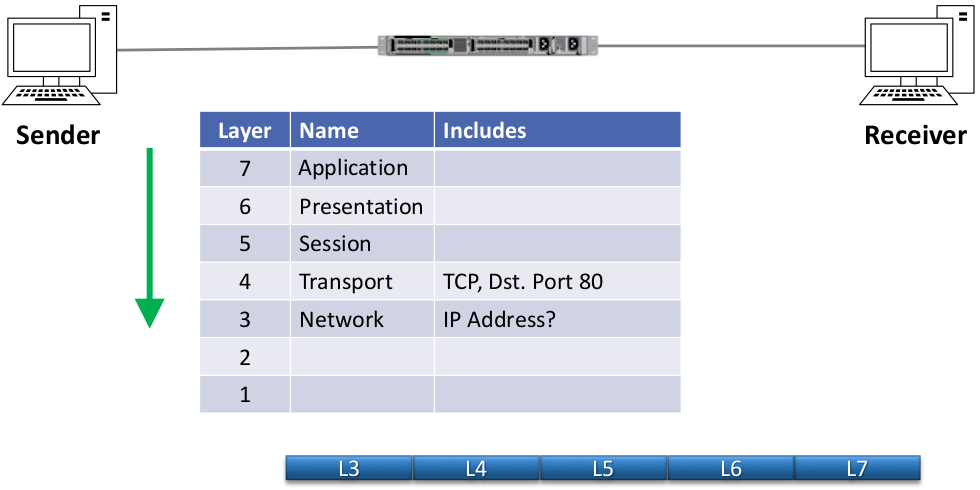
\includegraphics[width=\linewidth]{img/img40}
	\end{center}
\end{frame}

\begin{frame}{OSI Reference Model (Encapsulation)}
	\begin{center}
		\includegraphics[width=\linewidth]{img/img41}
	\end{center}
\end{frame}

\begin{frame}{OSI Reference Model (Encapsulation)}
	\begin{center}
		\includegraphics[width=\linewidth]{img/img42}
	\end{center}
\end{frame}

\begin{frame}{OSI Reference Model (Encapsulation)}
	\begin{center}
		\includegraphics[width=\linewidth]{img/img43}
	\end{center}
\end{frame}

\begin{frame}
	\frametitle{The Life of a Packet}
	\begin{center}
		\includegraphics[width=\linewidth]{img/img44}
	\end{center}
\end{frame}

\begin{frame}{The Life of a Packet}
	\begin{itemize}
		\item Switch 1 will send the packet to Router A which it already has in its MAC address table
	\end{itemize}
\end{frame}

\begin{frame}{The Life of a Packet}
	\begin{center}
		\includegraphics[width=\linewidth]{img/img45}
	\end{center}
\end{frame}

\begin{frame}{The Life of a Packet}
	\begin{itemize}
		\item Router A will receive the packet with destination IP address 10.10.12.10
		\item Router A does not have any interfaces in the 10.10.12.0/24 subnet
		\item In this case it will need a route to get there
		\item The route can be either statically configured by an administrator or learned dynamically through a routing protocol
	\end{itemize}
\end{frame}

\begin{frame}{The Life of a Packet}
	\begin{itemize}
		\item In this example the administrator has configured a static route for 10.10.12.0/24 with the next hop address 10.10.11.2
		\item Router A has an Ethernet interface in the 10.10.11.0 subnet
		\item It doesn’t know the MAC address for the next hop address 10.10.11.2 yet
		\item It will hold the HTTP packet and send an ARP request for 10.10.11.2
	\end{itemize}
\end{frame}

\begin{frame}{The Life of a Packet}
	\begin{center}
		\includegraphics[width=\linewidth]{img/img46}
	\end{center}
\end{frame}

\begin{frame}{The Life of a Packet}
	\begin{itemize}
		\item The ARP request will hit Router B’s interface 10.10.11.2
		\item Router B will process the ARP request and see it is for itself
		\item Router B will send a unicast ARP reply to Router A
		\item Router B will add an entry for Router A mapping IP address 10.10.11.1 to MAC address 5555.6666.7777 to its ARP cache
	\end{itemize}
\end{frame}

\begin{frame}{The Life of a Packet}
	\begin{center}
		\includegraphics[width=\linewidth]{img/img47}
	\end{center}
\end{frame}

\begin{frame}{The Life of a Packet}
	\begin{itemize}
		\item Router A will forward the HTTP packet it was holding to Router B
	\end{itemize}
\end{frame}

\begin{frame}{The Life of a Packet}
	\begin{center}
		\includegraphics[width=\linewidth]{img/img48}
	\end{center}
\end{frame}

\begin{frame}{The Life of a Packet}
	\begin{itemize}
		\item Router B will receive the HTTP packet and see that the destination IP address is 10.10.12.10
		\item Router B has an interface in the subnet 10.10.12.0/24, so it knows the destination should be available out that port
		\item It doesn’t know the MAC address of 10.10.12.10 so it will hold the HTTP packet and send an ARP request out of the 10.10.12.1 interface
	\end{itemize}
\end{frame}

\begin{frame}{The Life of a Packet}
	\begin{center}
		\includegraphics[width=\linewidth]{img/img49}
	\end{center}
\end{frame}

\begin{frame}{The Life of a Packet}
	\begin{itemize}
		\item The ARP request will be received by Switch 2
		\item Switch 2 will add an entry in its MAC address table mapping Router B’s MAC address 7777.8888.9999 to Port 1
		\item Switch 2 will flood the broadcast traffic out all ports apart from the one it was received on
	\end{itemize}
\end{frame}

\begin{frame}{The Life of a Packet}
	\begin{center}
		\includegraphics[width=\linewidth]{img/img50}
	\end{center}
\end{frame}

\begin{frame}{The Life of a Packet}
	\begin{itemize}
		\item The ARP request will hit the Web Server’s interface 10.10.12.10
		\item The Web Server will process the ARP request and see it is for itself
		\item The Web Server will send a unicast ARP reply to Router B
		\item The Web Server will add an entry for Router B mapping IP address 10.10.12.1 to MAC address 7777.8888.9999 to its ARP cache
		\item It will use this whenever it needs to send traffic to another IP subnet
	\end{itemize}
\end{frame}

\begin{frame}{The Life of a Packet}
	\begin{center}
		\includegraphics[width=\linewidth]{img/img51}
	\end{center}
\end{frame}

\begin{frame}{The Life of a Packet}
	\begin{itemize}
		\item Switch 2 will add an entry in its MAC address table mapping the Web Server’s MAC address 2222.3333.4444 to Port 2
		\item Switch 2 will send the ARP reply out only Port 1 which Router B is plugged into (which it already has in its MAC address table)
	\end{itemize}
\end{frame}

\begin{frame}{The Life of a Packet}
	\begin{center}
		\includegraphics[width=\linewidth]{img/img52}
	\end{center}
\end{frame}

\begin{frame}{The Life of a Packet}
	\begin{itemize}
		\item Router B will add an entry for the Web Server mapping IP address 10.10.12.10 to MAC address 2222.3333.4444 to its ARP cache
		\item Router B will send the HTTP request it was holding to the Web Server
	\end{itemize}
\end{frame}

\begin{frame}{The Life of a Packet}
	\begin{center}
		\includegraphics[width=\linewidth]{img/img53}
	\end{center}
\end{frame}

\begin{frame}{The Life of a Packet}
	\begin{itemize}
		\item Switch 2 will send the HTTP request out only Port 2 which the Web Server is plugged into (which it already has in its MAC address table)
	\end{itemize}
\end{frame}

\begin{frame}{The Life of a Packet}
	\begin{center}
		\includegraphics[width=\linewidth]{img/img54}
	\end{center}
\end{frame}

\begin{frame}
	\frametitle{OSI Reference Model\\(De-encapsulation)}
	\begin{center}
		\includegraphics[width=\linewidth]{img/img55}
	\end{center}
\end{frame}

\begin{frame}{OSI Reference Model\\(De-encapsulation)}
	\begin{center}
		\includegraphics[width=\linewidth]{img/img56}
	\end{center}
\end{frame}

\begin{frame}{OSI Reference Model\\(De-encapsulation)}
	\begin{center}
		\includegraphics[width=\linewidth]{img/img57}
	\end{center}
\end{frame}

\begin{frame}{OSI Reference Model\\(De-encapsulation)}
	\begin{center}
		\includegraphics[width=\linewidth]{img/img58}
	\end{center}
\end{frame}

\begin{frame}{OSI Reference Model\\(De-encapsulation)}
	\begin{center}
		\includegraphics[width=\linewidth]{img/img59}
	\end{center}
\end{frame}

\begin{frame}{OSI Reference Model\\(De-encapsulation)}
	\begin{center}
		\includegraphics[width=\linewidth]{img/img60}
	\end{center}
\end{frame}

\begin{frame}{OSI Reference Model\\(De-encapsulation)}
	\begin{center}
		\includegraphics[width=\linewidth]{img/img61}
	\end{center}
\end{frame}

\begin{frame}
	\frametitle{The Life of a Packet}
	\begin{itemize}
		\item The ARP and MAC addresses tables are already built so subsequent packets in either direction will flow without any need for ARP requests
		or switch flooding
	\end{itemize}
\end{frame}

\begin{frame}{The Life of a Packet}
	\begin{center}
		\includegraphics[width=\linewidth]{img/img62}
	\end{center}
\end{frame}

\begin{frame}{The Life of a Packet}
	\begin{center}
		\includegraphics[width=\linewidth]{img/img63}
	\end{center}
\end{frame}

\begin{frame}{The Life of a Packet}
	\begin{center}
		\includegraphics[width=\linewidth]{img/img64}
	\end{center}
\end{frame}

\end{document}
